\documentclass{article}
\usepackage{amsmath,amssymb}
\usepackage{hyperref}
\usepackage{graphicx}
\usepackage{listings}
\title{\bf{Turbine Formulation}}
\author{Nicholas Malaya, Roy Stogner, Robert D. Moser \\ Institute for
Computational Engineering and Sciences \\ University of Texas at Austin}
\date{} 

\begin{document}
\maketitle
\newpage
\section{Turbine Definitions}

The normal in the blade's velocity direction is, 
\begin{equation}
n_B = \frac{u_B}{||u_B||}. 
\end{equation}
Where $u_B$ is the blade velocity and is specified.
The normal in the fan vertical direction is also set, and is typically, 
\begin{equation}
n_v = \left(0,0,1\right)
\end{equation}
e.g. pointing ``up''. Then the normal in the radial direction must be, 
\begin{equation}
n_r = n_B \times n_v. 
\end{equation}
% The fan-wing-plane bit means that we're only looking at the projection
% of velocity into the plane that's defined by the base velocity and
% vertical direction. 

% (01:03:44 PM) Roy Stogner: The "local relative velocity" means that
% we're taking the velocity not in the reference frame of the domain, but
% in the reference frame of the wing.  So if the base velocity is U_B and
% the air velocity is U, then the local relative velocity is U - U_B. 
% (01:04:25 PM) Roy Stogner: Note that we simplify that equation a tiny
% bit by using the fact that U_B and N_R are perpendicular. 

Then, the fan-wing-plane component (e.g. the plane perpendicular to the 
radius) of local relative velocity is
\begin{equation}
u_p = u - (u\cdot n_r)\cdot n_r - u_B. 
\end{equation}
We can now define the lift and drag normals, where the direction
opposing drag is, 
\begin{equation}
n_{\text{drag}} = \frac{u_p}{||u_p||} 
\end{equation}
and the direction opposing lift orthogonal to the drag and the radial direction, 
\begin{equation}
n_{\text{lift}}= n_{\text{drag}} \times n_r. 
\end{equation}
Now the ``forward velocity'' in the reference frame of the turbine is, 
\begin{equation}
u_{\text{fwd}}= -u_p \cdot n_B
\end{equation}
and the ``upward'' velocity in this frame is, 
\begin{equation}
u_{\text{up}} = u_p \cdot n_v. 
\end{equation}
Finally, we can specify the angle with respect to the fan velocity
direction as, 
\begin{equation}
 \theta_f = \text{atan2}\left(\frac{u_{\text{up}}}{u_{\text{fwd}}}\right)
 %\theta_f = \text{tan}^{-1}\left(\frac{u_{\text{up}}}{u_{\text{fwd}}}\right)
\end{equation}
while the angle with respect to the chord is this with the addition of
the angle of attack of the blade, 
\begin{equation}
 \theta = \theta_f + \alpha(r).
\end{equation}
Now, we only need the drag polars in order to fully specify the force
on the blades.

\newpage
\section{Drag Polars}

We have been provided lift and drag as a function of angle of attack for
two cases, the flat plate and semi-circle turbine blades. 
For the flat plate, the drag polars are specified as,

\begin{lstlisting}
    theta := ((t+pi/2)%pi)-pi/2; 
    lift   = 'if(abs(theta)<pi/24,theta*9,sin(2*theta))'
    drag   = 'if(abs(theta)<pi/24,0.005+theta*theta*81/25,1-0.8*cos(2*theta))'
\end{lstlisting}
for example. 

\begin{figure}[!htb]
  \begin{center}
    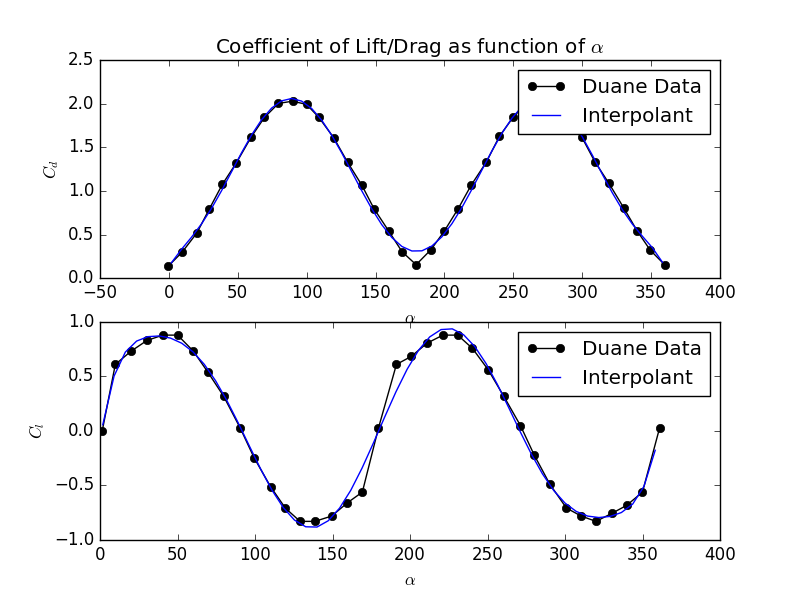
\includegraphics[width = 12 cm]{figs/flat}
    \caption{The flat plate interpolation.} 
    \label{flat}
  \end{center}
\end{figure}
As shown in Figure \ref{flat}, the fit is largely accurate. 

The semi-circular plots are more complicated. Here, we use a high order
polynomial fit to continuously interpolate between drag polars. This
results in a 
\begin{figure}[!htb]
  \begin{center}
    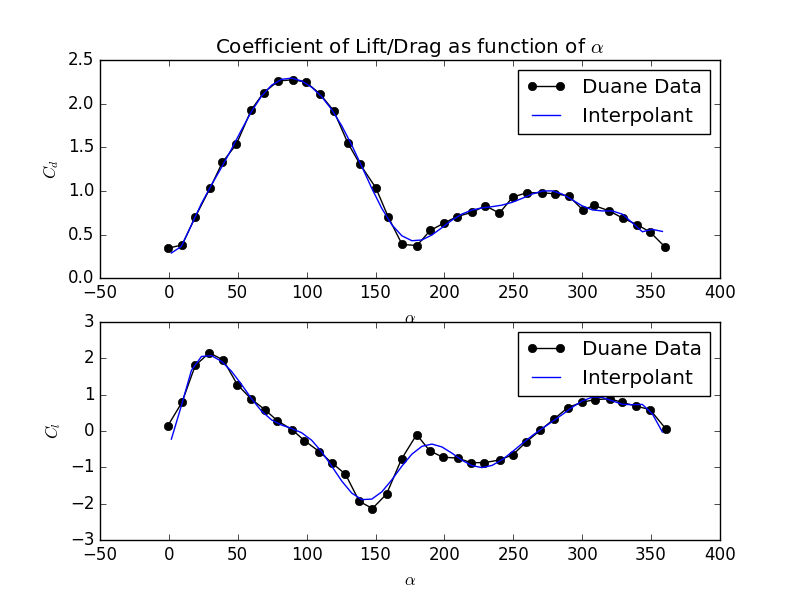
\includegraphics[width = 12 cm]{figs/semi}
    \caption{The semi-circular plate interpolation.} 
    \label{semi}
  \end{center}
\end{figure}
As shown in Figure \ref{semi}, the fit is decent, but not remarkably accurate.

Then, the force on the turbine is, 
\begin{equation}
 \boxed{F = \frac{1}{2}\frac{\rho u_p^2 C}{A}\left(C_l \cdot
					      n_\text{lift} + C_d \cdot n_\text{drag}  \right)}
\end{equation}

Where C is the chord length (specified as input), and A is the area,
which is also specified. For instance, the area swept might be, 
\begin{lstlisting}
     area_swept = '{r:=sqrt(x^2+y^2); 2*pi*r*(.6-.4)/4}'
\end{lstlisting}
for a 4 blade fan. The chord is specified similarly, for instance, 
\begin{lstlisting}
     chord_length = '.2*sqrt(2)'
\end{lstlisting}
would set a 0.28 meter chord length. 
%
% ---------------------------------------------------
% old turbine discussion:
% ---------------------------------------------------

% The penalty function will be added to the navier-stokes as, 
% % \begin{align}
% %  \partial_t(\rho u) = \text{NS} &+ \frac{1}{\epsilon}(u-u_t)\cdot n_p \\
% %                                 &+ \frac{1}{\epsilon}(u-\omega u_t)\cdot n_p \\
% % \end{align}

% \begin{align}
%  \partial_t(\rho u) = \text{NS} + \frac{1}{\epsilon}(u-\omega u_t)\cdot n_p
% \end{align}

% We will start by formulating a constant rotation speed
% turbine. The rotor will have counter-clockwise spin with angular
% velocity omega.   

% \begin{verbatim}
%   base_velocity=
%                 '{(r<r_max)*(z<zmax) * r * -sin(theta)*omega}
%                  {(r<r_max)*(z<zmax) * r * cos(theta)*omega}
%                  {0}'
% \end{verbatim}
% There are a few problems with this formulation. One, in a turbine, the
% fluid velocity is not necessarily identical to the blade velocity. 
% The turbine speed can take a range of values, and is often quoted as the
% `tip-speed ratio'', $\lambda$, which is,
%  \begin{equation}
%   \lambda = \frac{\omega R}{v}.
%  \end{equation}
% Here, R is the radius of the turbine blades, omega the angular velocity,
%  and v is the velocity of the fluid. Values for $\lambda$ generate power
%  in the range of 0-16, and are typically between 4 and 14. 

% Zmax will be the height of the vanes, which is approximately 0.84 meters in the laboratory, 
% and 1.0795 meters for the two-meter SoV configuration. Rmax will be the inner diameter of the vanes. 

%
% ---------------------------------------------------
% old discussion on determining the rotation speed:
% ---------------------------------------------------
% We now need to choose $\omega$. At the Betz limit, the velocities will be
% $V_{\text{out}}/V_{\text{in}} = 1/3$. Furthermore, the control volume
% analysis implies that,
% \begin{equation}
%  V_{\text{turbine}} = \frac{1}{2}\left(V_{\text{in}} + V_{\text{out}} \right)
% \end{equation}
% then,
% \begin{align}
%  V_{\text{turbine}} &= \left(\frac{1}{2}\right) \left(\frac{4}{3}\right) V_{\text{in}} \\
%  &= \frac{2}{3} V_{\text{in}}.
% \end{align}
% Note this is not the velocity of the turbine, but the velocity of the
% fluid around the turbine. We can estimate the turbine speed from the
% ``tip-speed ratio'', $\lambda$, which is,
% \begin{equation}
%  \lambda = \frac{\omega R}{v}.
% \end{equation}
% Here, R is the radius of the turbine blades, omega the angular velocity,
% and v is the velocity of the fluid. Values for $\lambda$ generate power
% in the range of 0-16, and are typically between 4 and 14. Thus, our
% angular velocity of the turbine is, 
% \begin{equation}
%  \omega = \frac{ 2 V_{\text{in}}\lambda}{3 R_{\text{max}}}.
% \end{equation}

% ---------------------------------------------------
% refs
% ---------------------------------------------------

%
% https://github.com/grinsfem/grins/tree/master/src/physics/src
% https://github.com/grinsfem/grins/blob/master/src/physics/src/averaged_fan.C
% https://github.com/grinsfem/grins/blob/master/src/physics/src/averaged_fan_base.C#L120
% https://github.com/grinsfem/grins/blob/3f86653ab5ba01981193ccce142ea196d0a192de/src/physics/src/averaged_fan_base.C
% https://github.com/grinsfem/grins/blob/34e2fc1e7d7143e0080f81c67bd584ce1236e2c1/src/physics/include/grins/averaged_fan.h
% https://github.com/grinsfem/grins/blob/34e2fc1e7d7143e0080f81c67bd584ce1236e2c1/src/physics/include/grins/averaged_fan_base.h
%


\end{document}
